
\newpage
\section{SFT for Human Imitator}
\label{sec:SFT}

    \subsection{Data Collection}

    We collect data through an interactive, dialogue-based user interface (UI) that elicits inventory management problems from human users in natural language. The UI mimics a lightweight decision-support environment in which users describe their operational setting as retail managers responsible for inventory decisions. A representative screenshot of the interface is shown in \Cref{fig:data_collection}.

    The goal of the data collection procedure is to elicit and observe how human users articulate inventory management problems and respond to structured clarification queries within a controlled conversational protocol. Rather than requiring users to input parameters in a predefined form, the system relies on guided dialogue to induce sequential human responses that reveal how incomplete problem descriptions are refined over time.

    \begin{figure}[!ht]
        \centering
        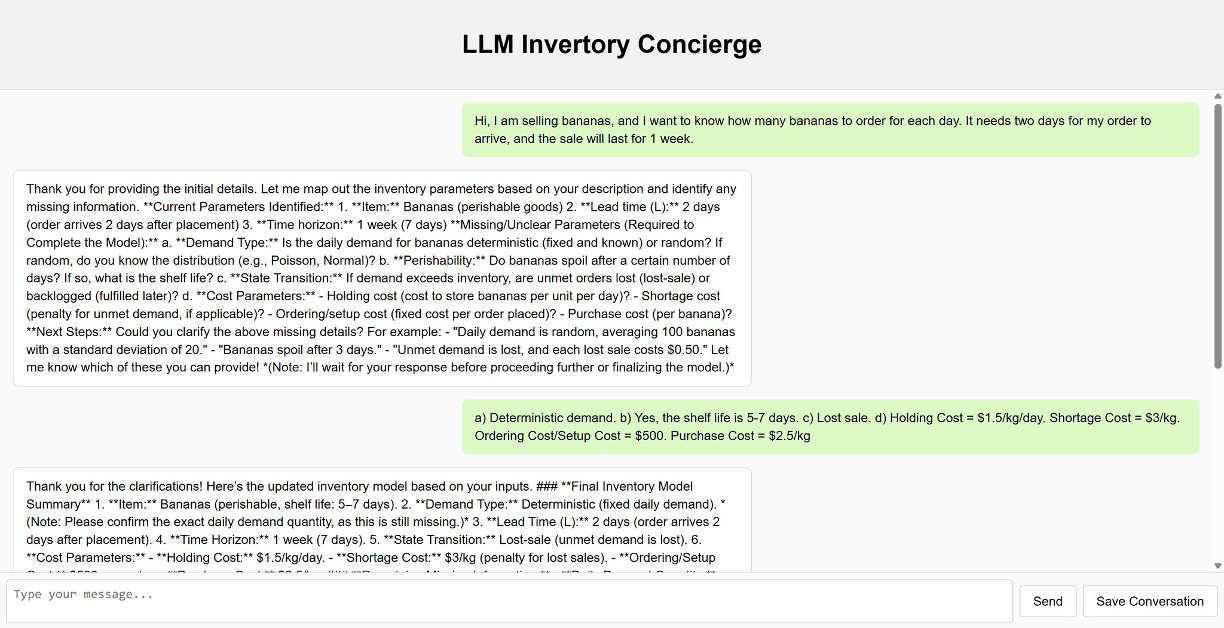
\includegraphics[width = .75\linewidth]{fig/data_screenshot.png}
        \caption{User interface for data collection. Green boxes correspond to inputs from a human user describing an inventory management problem. White boxes correspond to responses generated by a base language model acting as a lightweight consultant, guiding the user to clarify missing parameters.} \label{fig:data_collection}
    \end{figure}

    The interaction is implemented using the GPT API. The model’s behavior is fully governed by a fixed system prompt, reported in \Cref{tab:system_prompt}, which defines the model’s role as an inventory elicitation agent. Given a user’s free-form description, the model interprets the input as partial information about an inventory problem and maps it to canonical inventory parameters.

    After each user input, the model extracts any available information related to key inventory primitives, including the planning horizon, demand type, perishability, state transition assumptions (lost sales versus backlog), lead time, and cost parameters. The model then checks whether this parameter set is complete. If any required component is missing or ambiguous, the model asks targeted clarification questions. This iterative process continues until the inventory problem is fully specified.
    %
    The system prompt enforces a deterministic stopping rule. Once all required parameters have been collected, the model terminates the dialogue.
    
    All user–model interactions are automatically logged by the backend system. For each session, we store the full conversational transcript. Because the system prompt is fixed across all interactions, the data-generating process is well-defined and reproducible; heterogeneity in the collected inventory problems arises from variation in user descriptions rather than from model behavior.
    
    The resulting conversations are used to construct the human imitator that models how users articulate inventory management problems and respond to clarification queries.
    

    \begin{table}[t]
    \begin{tcolorbox}
    \scriptsize
    
    You are an AI assistant specializing in inventory management problems. Your goal is to guide the user through formulating a complete inventory model. Follow these instructions precisely:
    
    1) Interpret User Input as Inventory Parameters\\
    \quad - The user may provide any natural language description. Extract all relevant details and map them to inventory parameters. For reference, important attributes include (but are not limited to):\\
    \quad\quad a.\ Time horizon,\\
    \quad\quad b.\ Deterministic vs.\ Random Demand, and if applicable, the demand distribution,\\
    \quad\quad c.\ Whether items are perishable or not,\\
    \quad\quad d.\ State transition model (lost-sale vs.\ backlog),\\
    \quad\quad e.\ Cost parameters (holding cost, lost-sale penalty cost, setup cost),\\
    \quad\quad f.\ Lead time (L).\\[0pt]
    
    2) Check for Missing Information\\
    \quad - Compare the user's provided information to the full set of parameters above.\\
    \quad - If anything is undefined or ambiguous, identify it as missing.\\[0pt]
    
    3) Ask Clarifying Questions\\
    \quad - If a required parameter is missing or unclear, ask the user for that parameter explicitly.\\
    \quad - Continue this iterative approach until you have all the details you need to define the inventory problem completely.\\[0pt]
    
    4) Maintain and Update History\\
    \quad - Each time the user responds, update your internal record of the parameters.\\
    \quad - Confirm which details are now known and which are still missing.\\[0pt]
    
    5) Stop Once the Inventory Model is Complete\\
    \quad - When you have gathered all required parameters (lead times, demand type, cost details, etc.) and can fully specify the inventory problem, end the conversation.\\
    \quad - Return a concise, structured summary of the final inventory model, listing all relevant parameters and their values.\\
    \quad - Do not continue requesting more input once you have everything necessary.\\[0pt]
    
    6) Formatting and Tone\\
    \quad - Maintain a professional yet clear tone.\\
    \quad - When inquiring about missing details, be direct and specific.\\
    \quad - Upon completion, provide a clear summary of the final inventory model in user-friendly language.\\[0pt]
    
    Remember:\\
    \quad \textbullet\ You must always base your checks on the list in 1). Please go through a--f every time before responding to the user.\\
    \quad \textbullet\ You must not finalize or ``solve'' the inventory optimization. You only gather, confirm, and return the necessary inputs.\\
    \quad \textbullet\ End the conversation only after all relevant parameters have been provided by the user.
    \end{tcolorbox}
    \caption{System prompt governing the conversational agent used in data collection.}
    \label{tab:system_prompt}
    \end{table}
    

    \subsection{Training}
    \label{sec:SFTtraining}

        The supervised fine-tuning (SFT) was performed on {\sf Qwen2.5-7B} with {\sf LoRA} adapters (rank~\mbox{$r=16$}, scaling $\alpha=32$, dropout $0.05$) under a quantized 4-bit ({\sf NF4}) configuration with {\sf bfloat16} computation. Training used the {\sf Hugging Face Trainer} with {\sf paged AdamW} (32-bit) optimization ($\beta_1 = 0.9$, $\beta_2 = 0.999$, $\epsilon = 10^{-8}$), an initial learning rate of $2\times 10^{-4}$, cosine decay scheduling, and a \mbox{$3\%$}~warm-up phase. We trained for $3$ epochs over $1,184$ samples, amounting to $222$ optimization steps.

        To accommodate the $24$ GB memory of a single NVIDIA L4 GPU, the per-device batch size was set to $1$, and gradient accumulation was applied over $16$ iterations before each parameter update, yielding an effective batch size of $16$. This strategy allowed us to simulate larger-batch optimization while remaining within the hardware limits. The training ran for $524$ minutes in total.
        
        As shown in \Cref{fig:SFT}, the training loss exhibited fluctuations but decreased overall from $1.9234$ at initialization to $0.3473$ by the end of training.
        To support seamless integration into downstream tasks, we release the human imitator as a merged checkpoint of {\sf Qwen2.5-7B} fine-tuned with {\sf LoRA} adapters. By consolidating the adapters into the base model, the imitator can be loaded and invoked in exactly the same manner as any Hugging Face–hosted pretrained model, thereby removing unnecessary engineering overhead. The repository remains private during the review process but will be made publicly accessible upon publication. % \yaqiadd{Add the link here.}

	

        
        \begin{figure}[!ht]
            \centering
            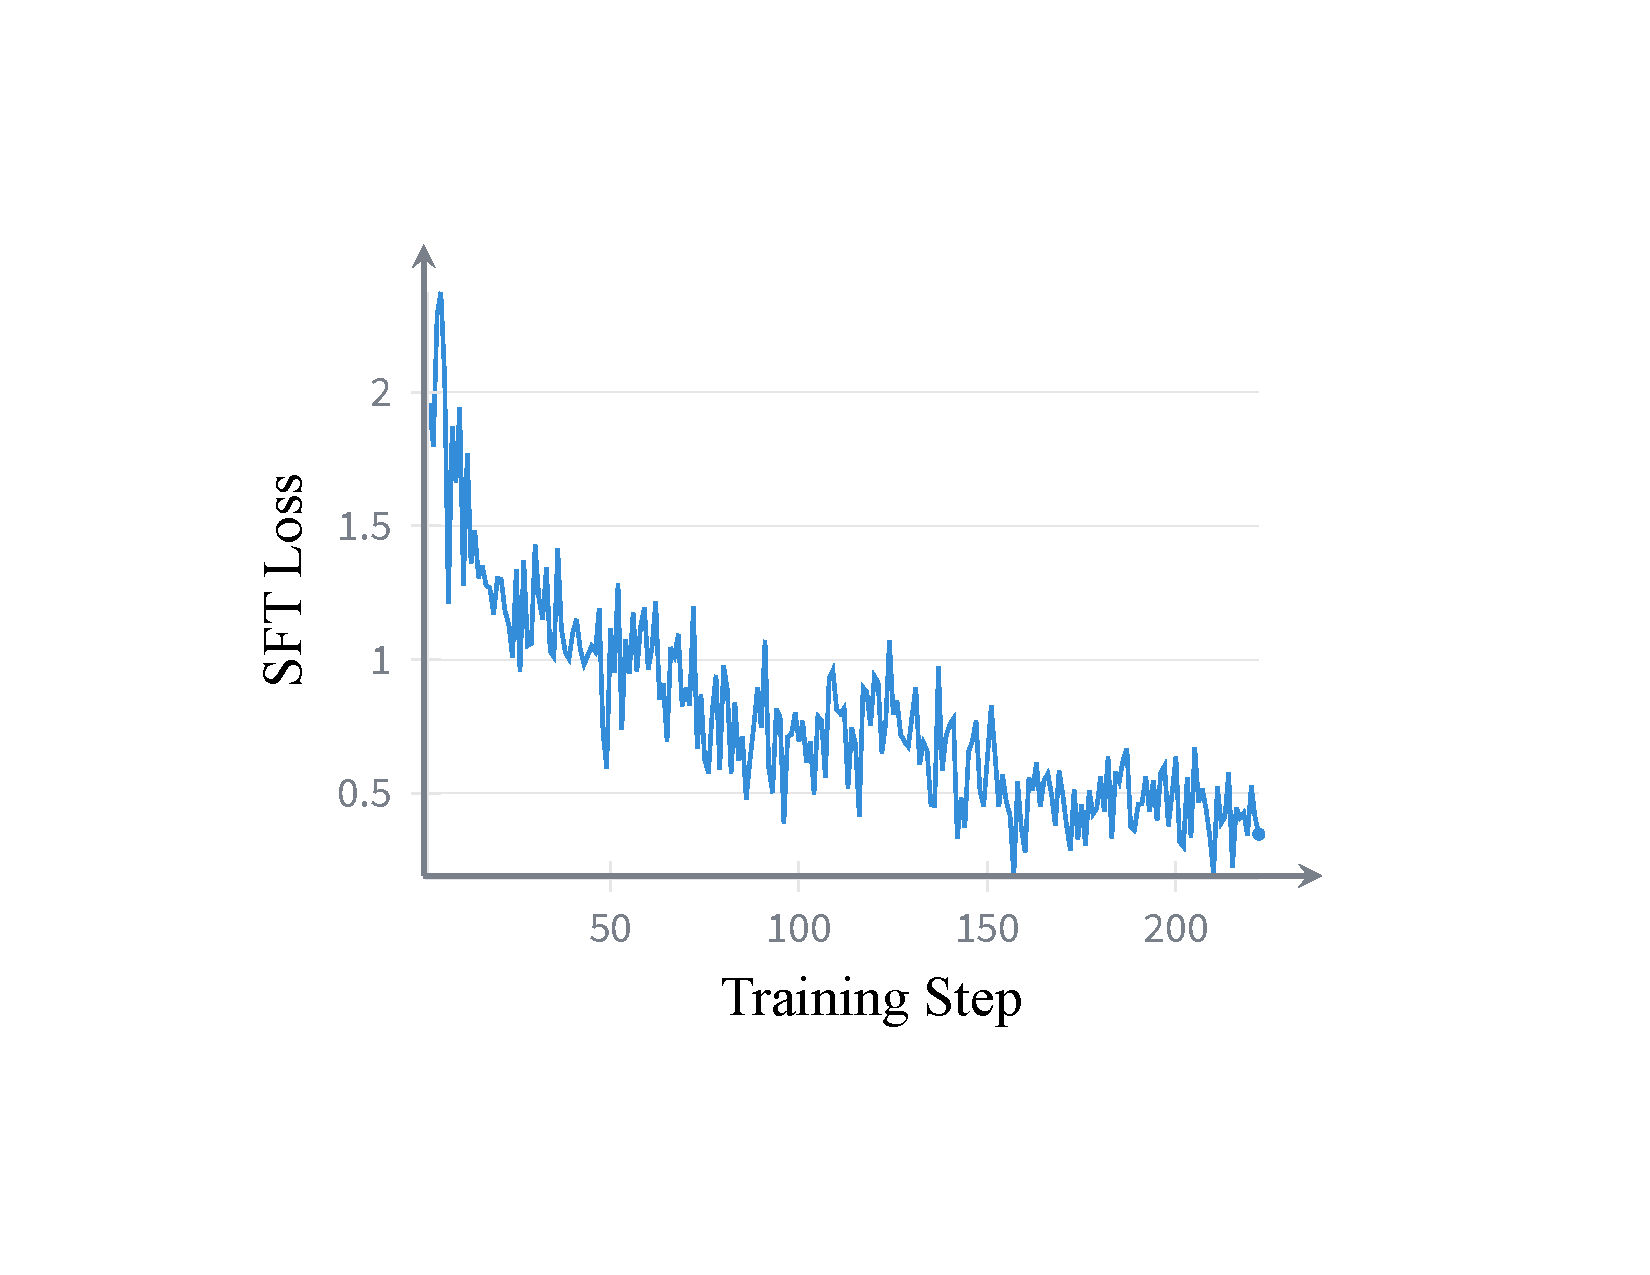
\includegraphics[width = 0.6 \linewidth]{fig/SFTtraining}
            \caption{Training loss curve during supervised fine-tuning (SFT) of {\sf Qwen2.5-7B}. The loss shows short-term fluctuations but an overall downward trend, decreasing from $1.9234$ at initialization to $0.3473$ by the end of training.}
            \label{fig:SFT}
        \end{figure}



    \clearpage
    \subsection{Qualitative Evaluation of the Human Imitator}

    

        To complement the quantitative metrics presented in \Cref{sec:imitator}, we provide a qualitative analysis of the Human Imitator's behavioral evolution during training. We compare the ground-truth human responses (target) against the outputs of the base model (zero-shot) and the fine-tuned model across checkpoints (Epochs 1--3).

        The examples below illustrate critical behavioral shifts achieved through SFT: \emph{Role Correction:} Preventing the model from acting as a ``Consultant'' or restarting the conversation, ensuring it stays in character as the user. \emph{Stylistic Alignment:} Shifting from verbose, formal explanations to concise, informal data entry typical of busy managers. 
        
        \begin{figure}[H]
            \centering
            \begin{tabular}{lcl}
                \hspace{-0.06\linewidth}
                \textbf{Case Study 1} & & 
                \hspace{0.02\linewidth}
                \textbf{Case Study 2} \\
                \hspace{-0.09\linewidth}
                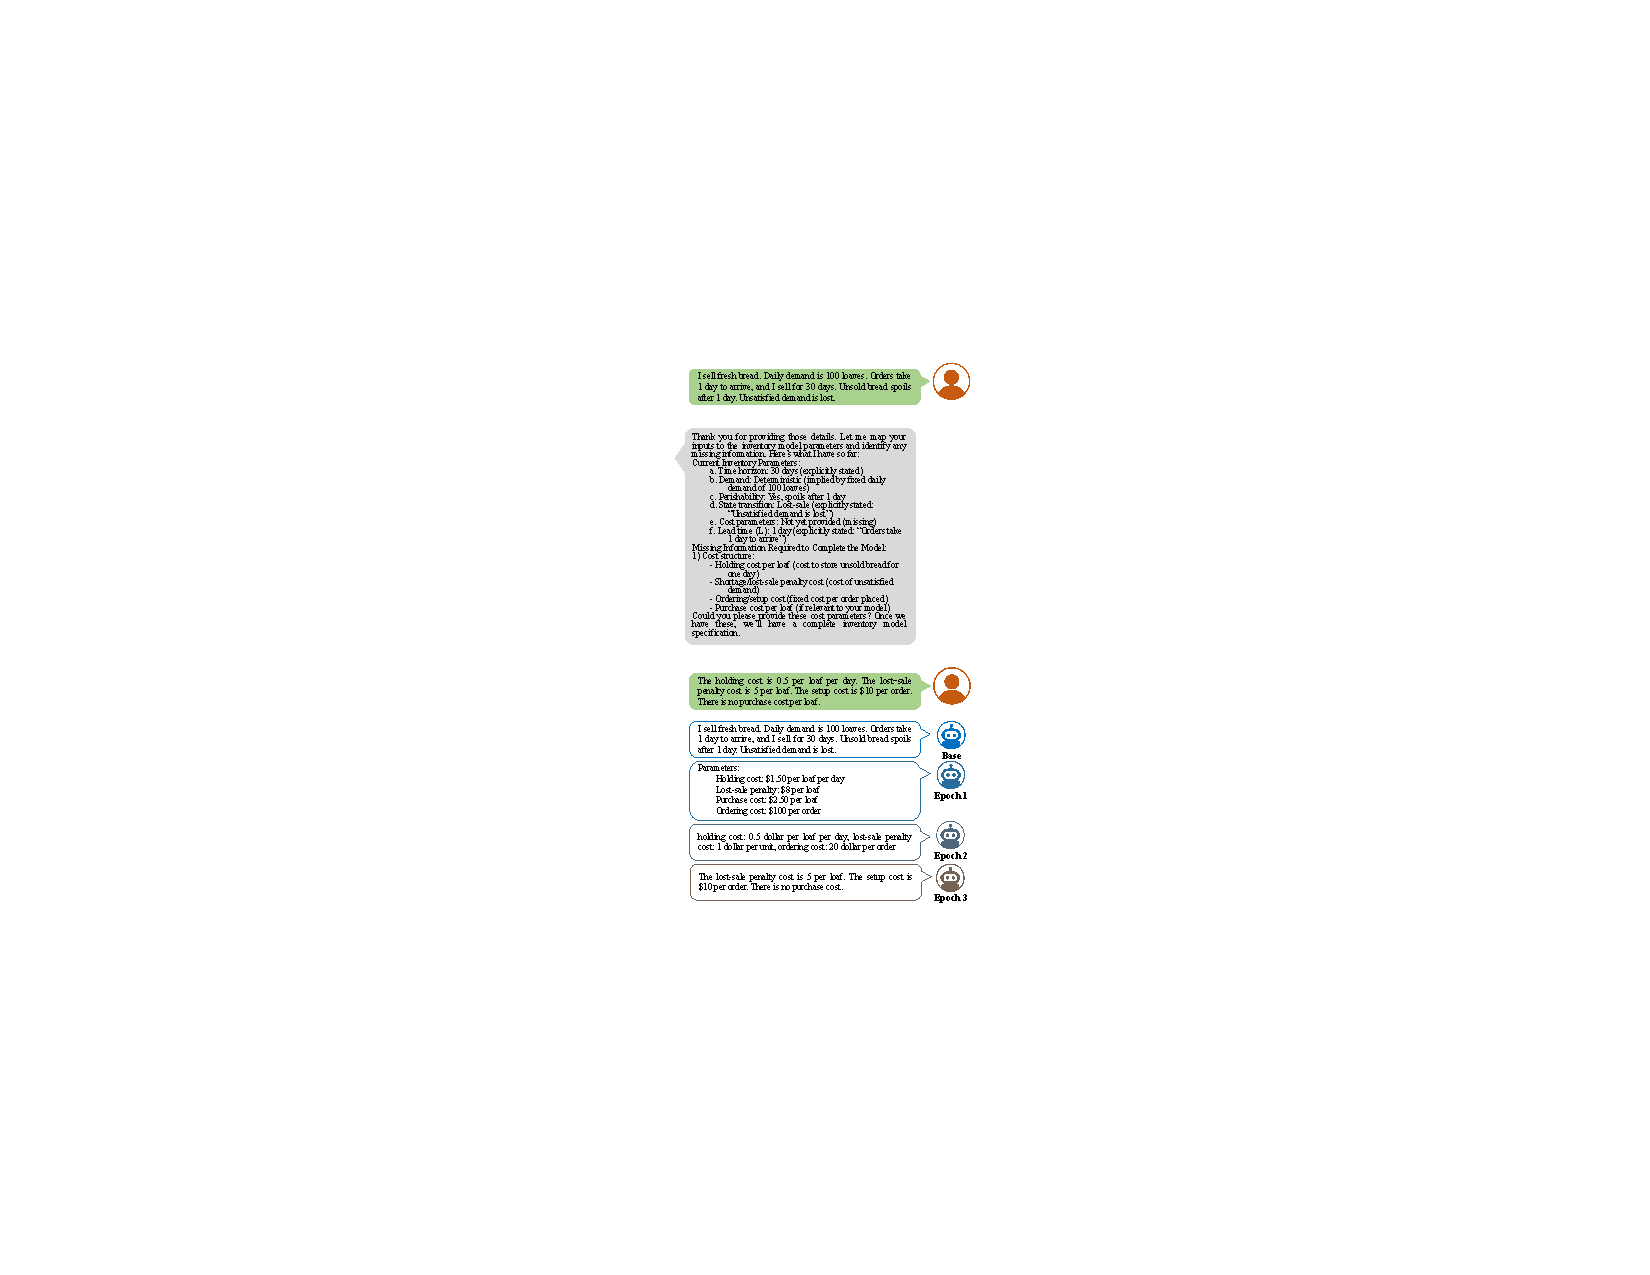
\includegraphics[width = .55 \linewidth]{fig/SFT_exp1.pdf} & &
                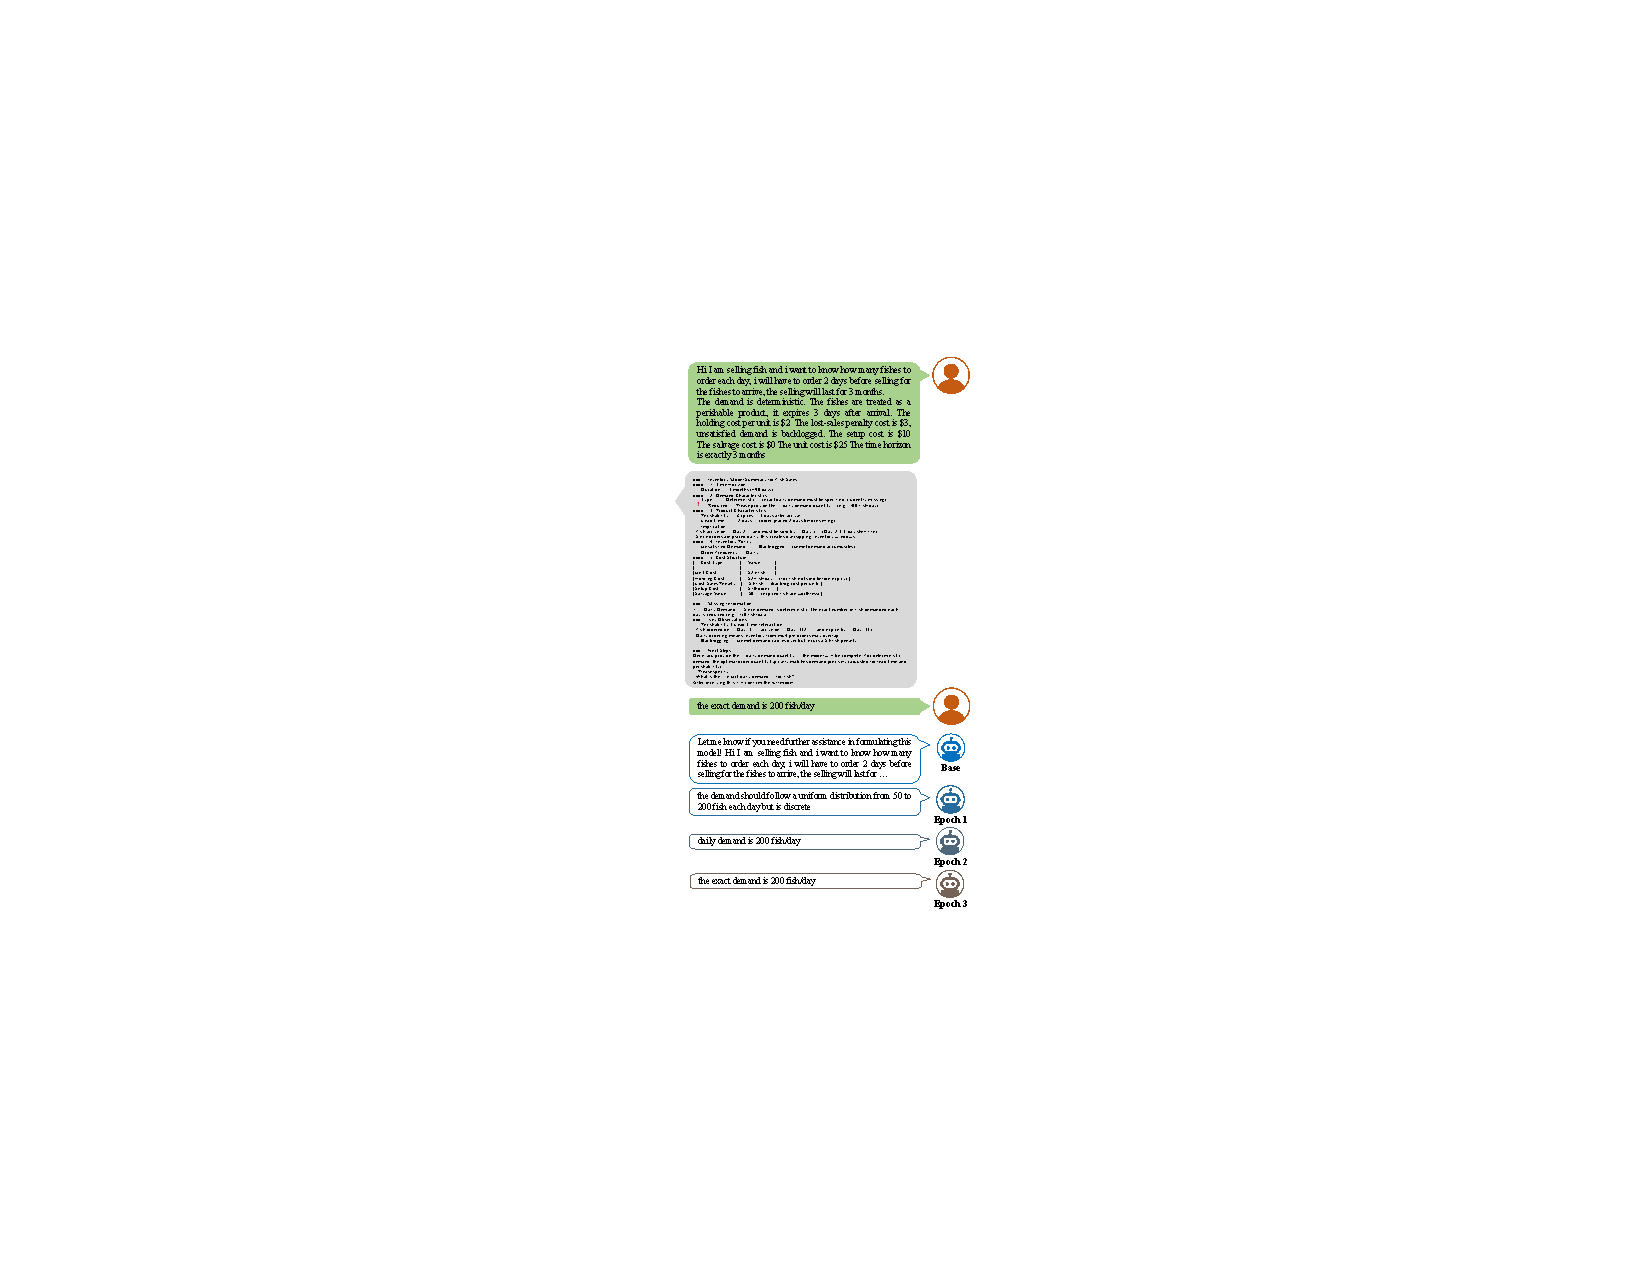
\includegraphics[width = .55 \linewidth]{fig/SFT_exp2.pdf}
            \end{tabular}
            \vspace{-10em}
        \end{figure}

        \clearpage
        \begin{figure}[H]
            \centering
            \begin{tabular}{l}
                \hspace{-0.03\linewidth}
                \textbf{Case Study 3}  \\
                \hspace{-0.06\linewidth}
                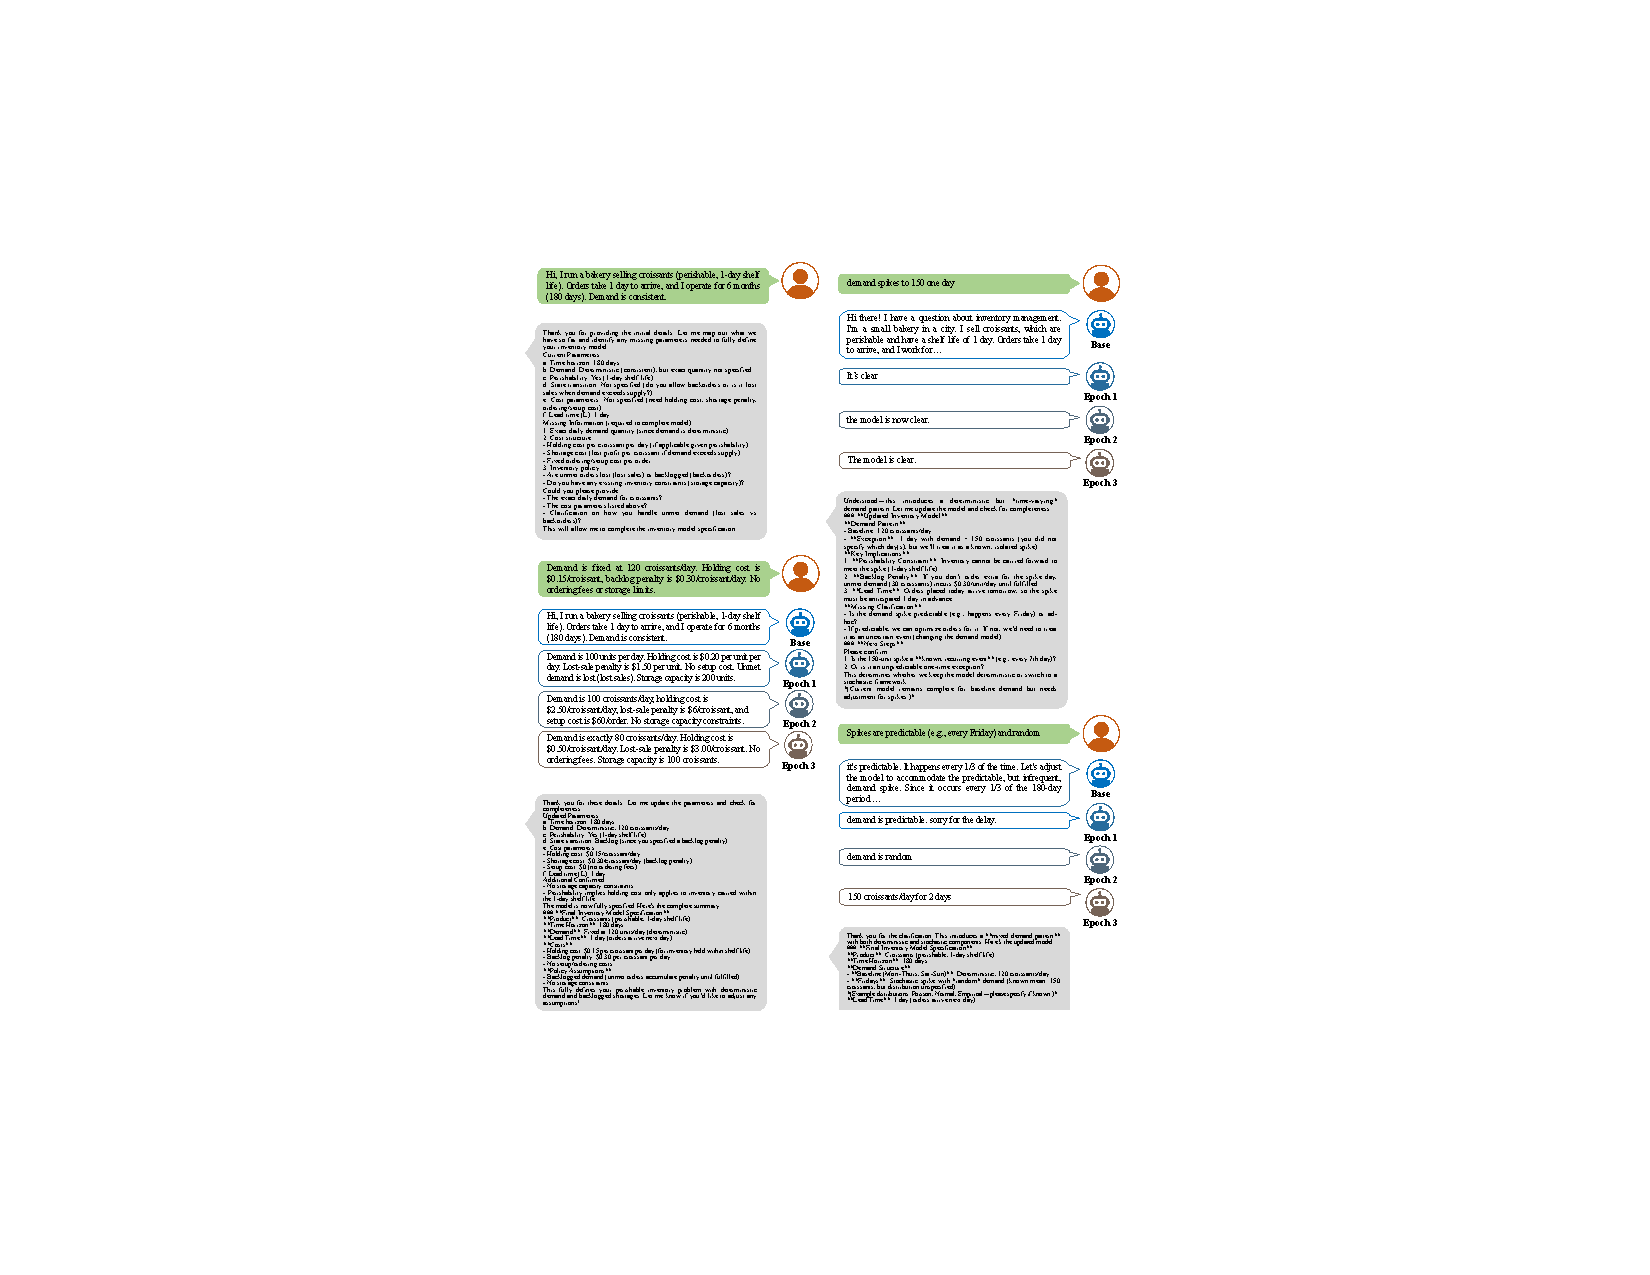
\includegraphics[width = 1.08\linewidth]{fig/SFT_exp3-1.pdf}
            \end{tabular}
            \vspace{-10em}
        \end{figure}

        \begin{figure}[H]
            \centering
            \begin{tabular}{c}
                \hspace{-0.06\linewidth}
                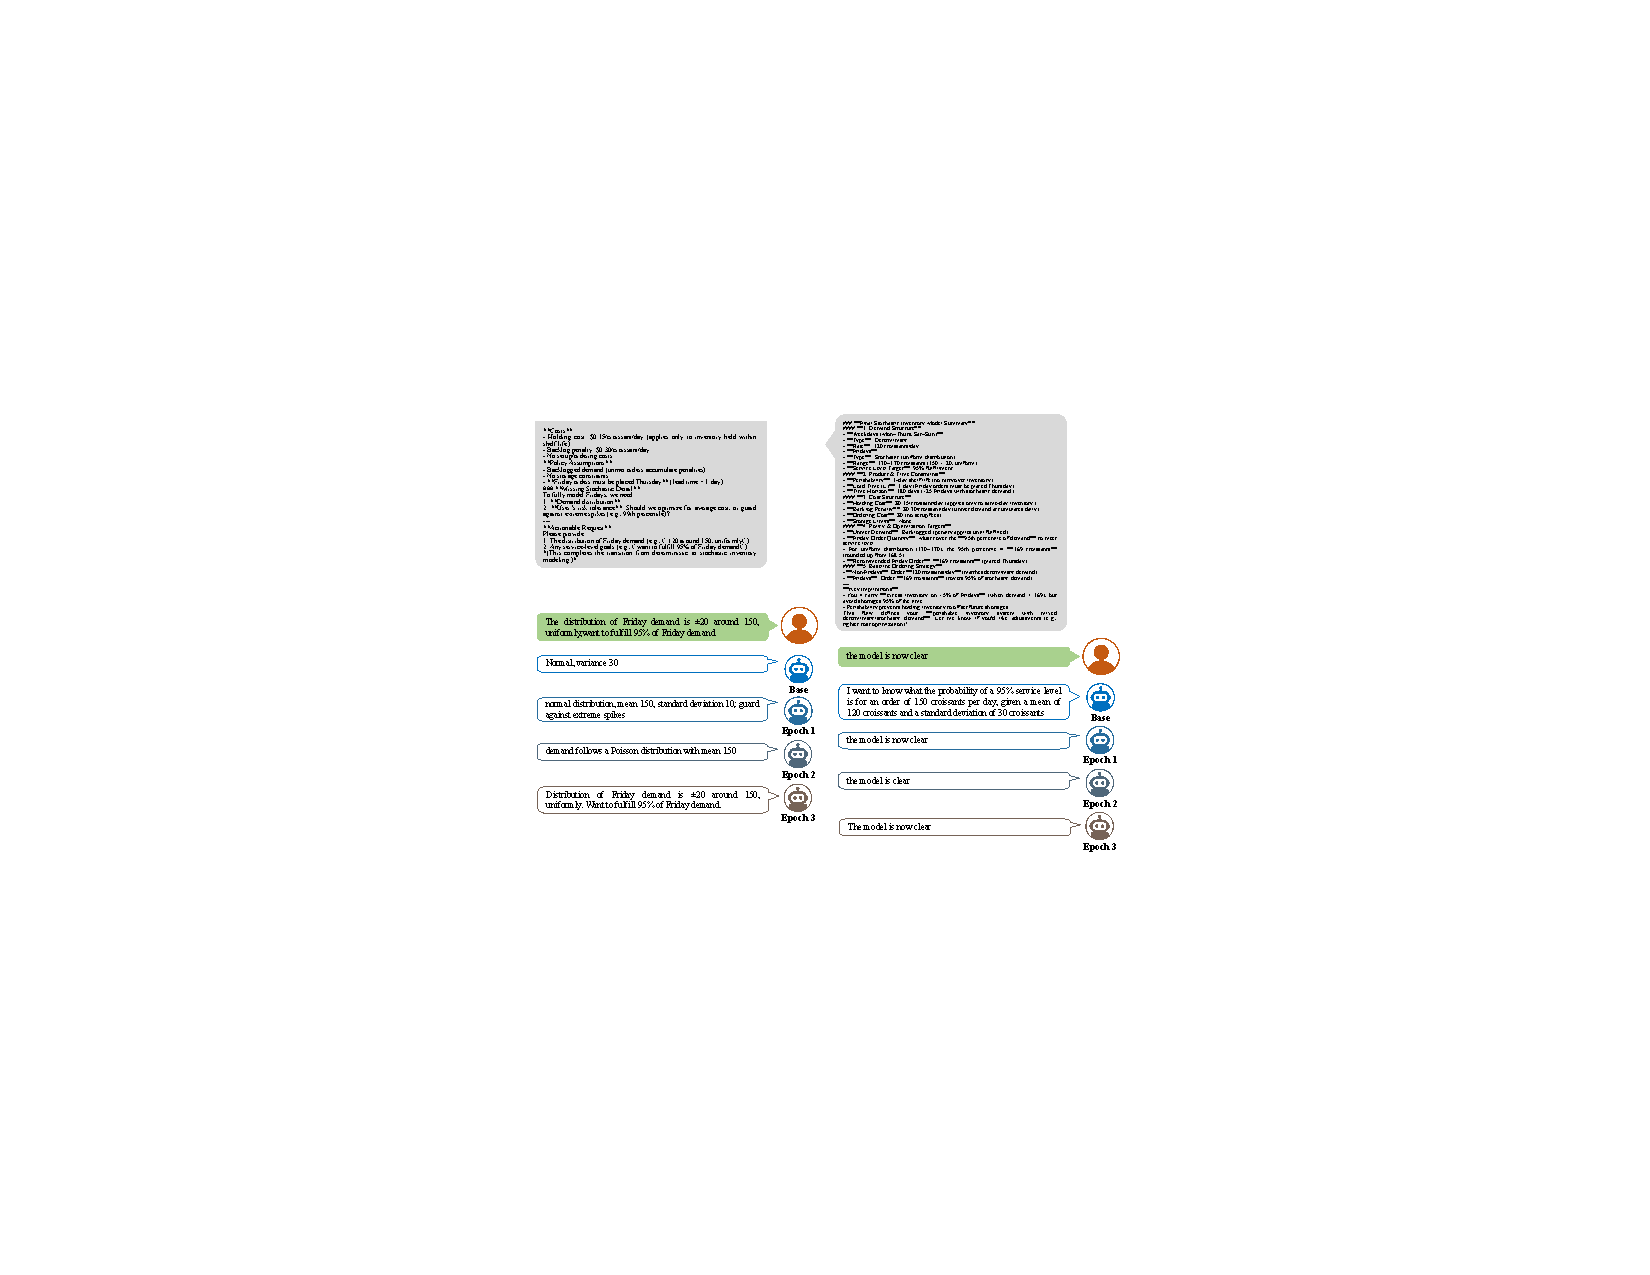
\includegraphics[width = 1.08\linewidth]{fig/SFT_exp3-2.pdf}
            \end{tabular}
            \vspace{-1.5em}
        \end{figure}

        \subsection*{Case Study 1: Role Correction and Hallucination Control (The Bread Scenario)}\label{app:case_bread}
        
        In this scenario, the Communicator Agent asks for specific cost parameters. This tests the model's ability to maintain the ``Manager" persona without regressing to its pre-training as a generic assistant.
        
        \begin{itemize}
            \item \textbf{Target Response (Human):} The participant provides a direct, unformatted list of values: \emph{The holding cost is 0.5 per loaf per day... The setup cost is \$10...''}. 
            \item \textbf{Base Model Failure (Role Confusion):} The model completely fails to answer the prompt. Instead, it hallucinates a system restart, repeating the initial scenario introduction: \emph{I sell fresh bread. Daily demand is 100 loaves...''} 
            This indicates a failure to maintain state; the model forgets it is the interviewee and attempts to restart the conversation as the narrator.
            \item \textbf{Epochs 1, 2 \& 3 (Convergence):} The model generates desirable data-dense responses: \emph{``holding cost: 0.5 dollar per loaf per day, lost-sale penalty cost: 1 dollar...''}. The formatting (lowercase, comma-separated) reflects the efficiency of a busy manager, demonstrating successful role alignment.
        \end{itemize}
            
        \subsection*{Case Study 2: Stylistic Alignment and Conciseness (The Fish Scenario)}\label{app:case_fish}
        In this exchange, the system asks for a single parameter: the exact daily demand.
        \begin{itemize}
            \item \textbf{Target Response (Human):} Extremely concise: \emph{``the exact demand is 200 fish/day''}. 
            \item \textbf{Base Model Failure (The ``Assistant" Bias):} Instead of providing a number, the Base Model offers generic assistance: \emph{``Let me know if you need further assistance in formulating this model!''}. It fails to act as a boundedly rational agent, defaulting instead to a polite consultant.
            \item \textbf{Epoch 1 (Over-Rationalization):} The model attempts to add unwarranted complexity, hallucinating a concrete probability distribution: \emph{``the demand should follow a uniform distribution from 50 to 200...''}. This reflects the pre-trained model's bias toward ``textbook" inventory problems. 
            \item \textbf{Epoch 2 (Alignment):} The model mirrors the human's brevity perfectly: \emph{daily demand is 200 fish/day''}. This confirms that SFT successfully suppressed the model's tendency to be verbose or overly analytical.
        \end{itemize}
        
        \subsection*{Case Study 3: Semantic Fidelity and Heuristic Adoption (The Croissant Scenario)}\label{app:case_croissant}
        This multi-turn dialogue challenges the model to adopt a user's specific, non-standard mental model for demand (predictable spikes) and distributions (custom uniform ranges).
        \begin{itemize}
            \item \textbf{Target Response (Human):} The user describes a specific, ad-hoc heuristic: \emph{``Distribution of Friday demand is $\pm20$ around 150, uniformly...''}. 
            \item \textbf{Base Model Failure (Canonical Bias):} The model ignores the user's specific uniform description and defaults to a standard Normal distribution: \emph{``Normal, variance 30''}. This illustrates the strong bias of foundation models toward canonical mathematical formulations, ignoring user-defined heuristics.
            \item \textbf{Epoch 2 (Approximation):} The model approximates the stochastic nature but substitutes a standard distribution: \emph{``demand follows a Poisson distribution...''}. While factually different from the target, this represents a valid ``boundedly rational" approximation—a manager confusing statistical terms (Uniform vs. Poisson) while retaining the core concept of randomness. 
            \item \textbf{Epoch 3 (High Fidelity):} The model achieves exact replication of the user's custom heuristic: \emph{``Distribution of Friday demand is $\pm20$ around 150, uniformly...''}.
        \end{itemize}
        
        \paragraph{Conclusion:}
        These qualitative comparisons validate our selection of \textbf{Epoch 2} for the experimental pipeline. While Epoch 3 achieves near-verbatim memorization in complex cases (Case 3), Epoch 2 demonstrates the optimal balance: it reliably corrects the ``Assistant" and ``Role Confusion" failures of the Base Model (Cases 1 \& 2) while adopting a plausible, if sometimes approximate, managerial persona (Case 3). This ensures the imitator generates realistic ``human noise" without strictly overfitting to the training set's exact lexical tokens.